\documentclass[10pt,a4paper, margin=1in]{article}
\usepackage{fullpage}
\usepackage{amsfonts, amsmath, pifont}
\usepackage{amsthm}
\usepackage{graphicx}
\usepackage{float}

\usepackage{tkz-euclide}
\usepackage{tikz}
\usepackage{pgfplots}
\pgfplotsset{compat=1.13}

\usepackage{geometry}
 \geometry{
 a4paper,
 total={210mm,297mm},
 left=10mm,
 right=10mm,
 top=10mm,
 bottom=16mm,
 }
 % Write both of your names here. Fill exxxxxxx with your ceng mail address.
 \author{
  Akçan, Batuhan\\
  \texttt{e2580181@ceng.metu.edu.tr}
  \and
  Sönmezer, Mert\\
  \texttt{e2516920@ceng.metu.edu.tr}
}

\title{CENG 384 - Signals and Systems for Computer Engineers \\
Spring 2024 \\
Homework 2}
\begin{document}
\maketitle



\noindent\rule{19cm}{1.2pt}

\begin{enumerate}

\item %write the solution of q1
    By looking at the graphs provided in the question, the equation of the functions are as follows:
    $$x(t)=u(t+3)-u(t-7)$$
    $$h(t)=u(t-1)-u(t-15)$$
    Then, $y(n)$ becomes
    $$y(n)=x(n)*h(n)$$
    $$y(n)=\int_{-\infty}^{\infty}x(\tau)h(t-\tau)$$
    $x(\tau)$ and $h(t-\tau)$ will
    \begin{itemize}
        \item partially overlap for $-2\leq t\leq 8$
        \item fully overlap for $8< t\leq 12$
        \item partially overlap for $12< t\leq 22$
    \end{itemize}
    We need to evaluate the convolution sum for these three regions separately.
    \[ y(t) = \begin{cases} 
          t+2 & -2\leq t\leq 8 \\
          10 & 8<t\leq 12 \\
          22-t & 12<t\leq 22\\
          0 & otherwise
       \end{cases}
    \]

\item %write the solution of q2  
	\begin{enumerate}
    % Write your solutions in the following items.
    \item %write the solution of q2a
    Notice that the overlapped part of the convolution process starts at the point $n=-4$ and ends at the point $n=4$, so for $n\leq -5$ and $n\geq 5$, $y_1[n]=0$. Now, let's calculate the convolution sum for every $n$ value in the interval.
    \begin{align*}
        n&=-4\rightarrow x[-4]h[-4]+x[0]h[0]=0+2=2 \\
        n&=-3\rightarrow x[-3]h[-3]+x[1]h[1]=0+0=0 \\
        n&=-2\rightarrow x[-2]h[-2]+x[2]h[2]=0+4 \\
        n&=-1\rightarrow x[-1]h[-1]+x[3]h[3]=0+0=0 \\
        n&=0\rightarrow x[0]h[0]+x[4]h[4]=1-6=-5 \\
        n&=1\rightarrow x[1]h[1]+x[5]h[5]=0+0=0 \\ 
        n&=2\rightarrow x[2]h[2]+x[6]h[6]=2+0=2 \\
        n&=3\rightarrow x[3]h[3]+x[7]h[7]=0+0=0 \\
        n&=4\rightarrow x[4]h[4]+x[8]h[8]=0-3=-3 \\
    \end{align*}
    Then, the graph of $y_1[n]$ will be like in Figure \ref{fig:q2a}
    \begin{figure}[htbp]
        \centering
            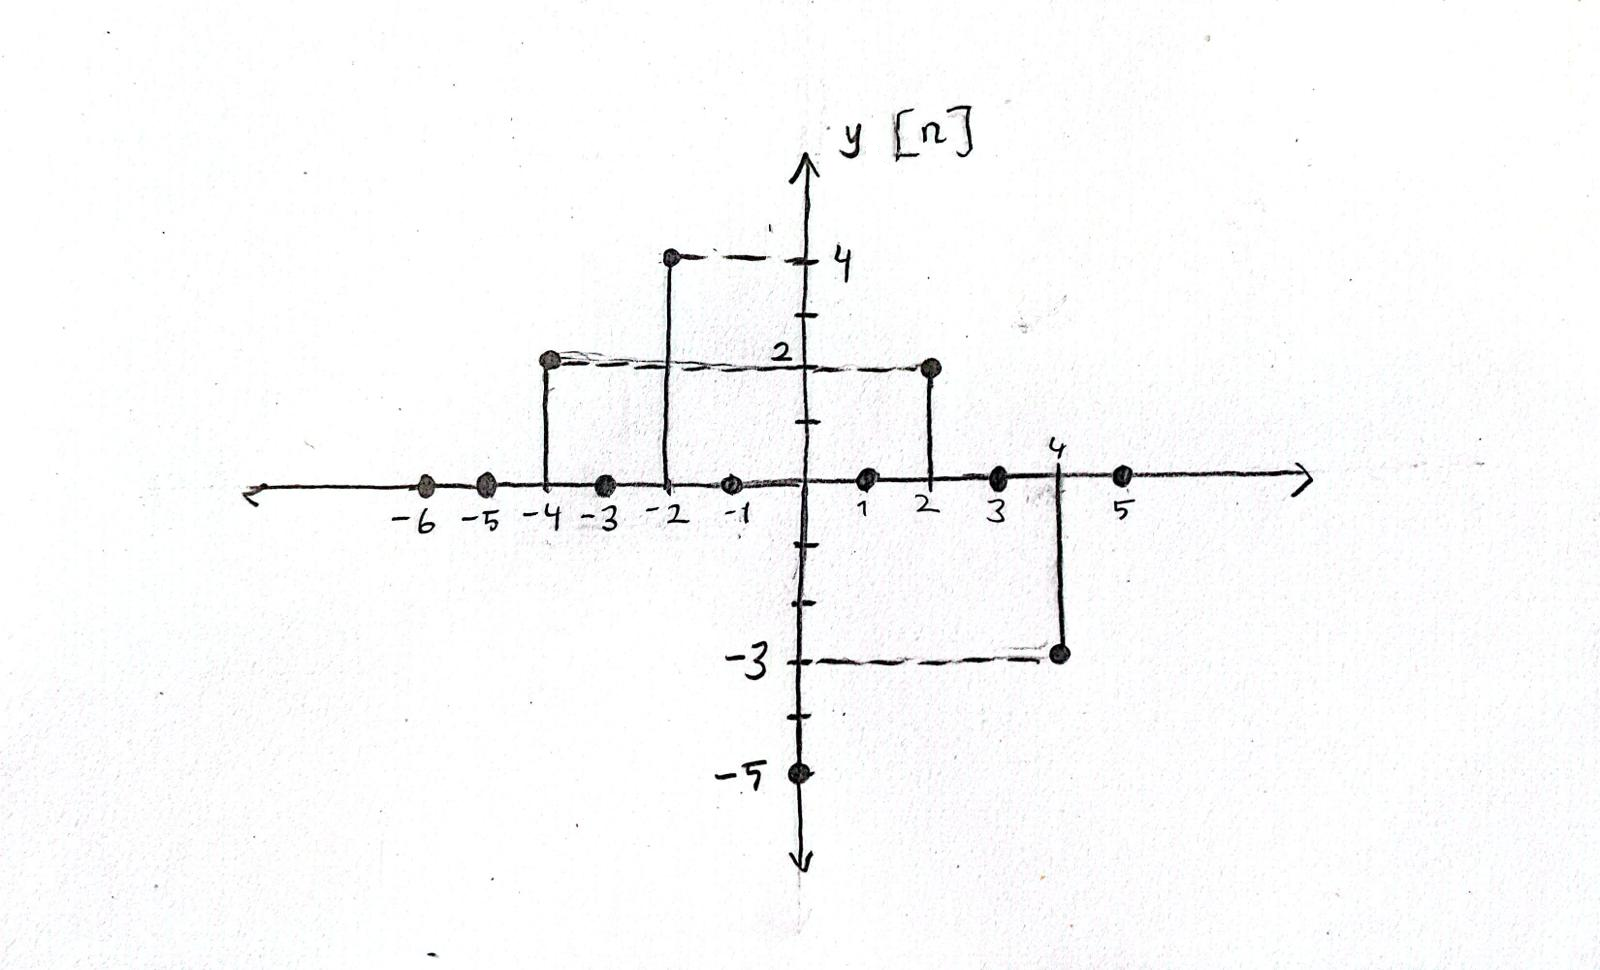
\includegraphics[scale=0.3]{q2a.jpg}
            \caption{The graph of $y_1[n]$.}
            \label{fig:q2a}
    \end{figure}
    
    \item %write the solution of q2b
    We know that the system is LTI. That's why sliding in the input should exactly be reflected to the output.
    \begin{align*}
        x[n] &\xrightarrow{LTI} y_1[n] \\
        x[n+2] &\xrightarrow{LTI} y_1[n+2] = y_2[n]
    \end{align*}
    Therefore, the output $y_2[n]$ will be as in Figure \ref{fig:q2b}:
    \begin{figure}[htbp]
        \centering
            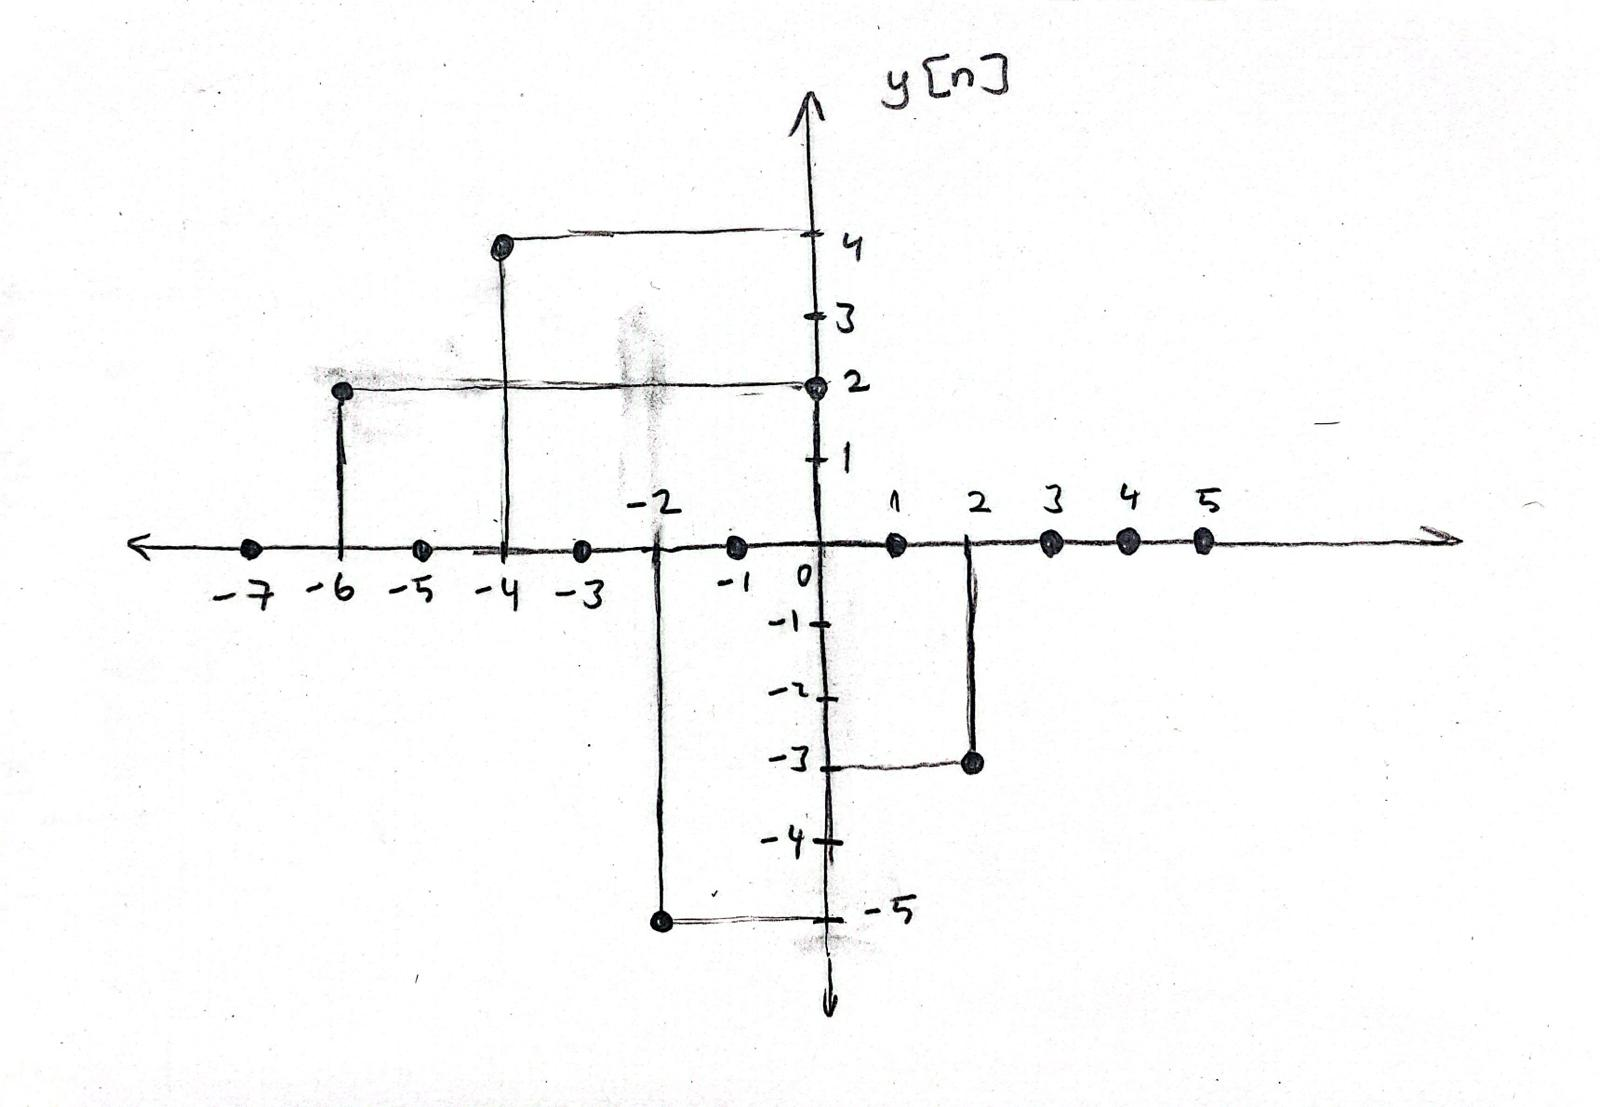
\includegraphics[scale=0.3]{q2b.jpg}
            \caption{The graph of $y_2[n]$.}
            \label{fig:q2b}
    \end{figure}
    
    \item %write the solution of q2c
    To compute $y_3[n]$, we first need to find $x[n+2]*h[n-2]$.
    $$y_3[n]=x[n+2]*h[n-2]=\sum_{k=-\infty}^{\infty}x[k+2]h[n-k-2]$$
    In the equation above, we can use the change of variable method. Let's define $m=k-2$. Then, the equation above will be as follows:
    $$y_3[n]=\sum_{m=-\infty}^{\infty}x[m]h[n-m]$$
    Notice that by looking at this equation, $y_3[n]$ is exactly same as $y_1[n]$. Therefore, the graph of $y_3[n]$ will be the same as Figure \ref{fig:q2a}
    \end{enumerate}

\item %write the solution of q3
    \begin{enumerate}
    % Write your solutions in the following items.
    \item %write the solution of q3a
    We need to replace $x[n]$ with $\delta [n]$. Then, $y[n]$ becomes $h[n]$, which is the impulse response of the system.
    $$h[n] = \frac{1}{5}\delta [n-1]+\delta[n]$$
    \item %write the solution of q3b
    To find the output $y[n]$ defined in the question, we need to replace $x[n]$ with $\delta [n-2]$.
    $$y[n] = \frac{1}{5}\delta [n-3]+\delta[n-2]$$
    \item %write the solution of q3c
    This system is BIBO stable because for any bounded input $x[n] < B$, we will get a bounded output. From another perspective, its impulse response is summable.
    $$\sum_{k=-\infty}^{\infty}|h[k]|=\sum_{k=-\infty}^{\infty}|\frac{1}{5}\delta [k-1]+\delta[k]|=\frac{1}{5}+1=\frac{6}{5}<\infty$$
    \item %write the solution of q3d
    This system has memory since $h[n] = K\delta [n]$. In other words, the first term, which is $\frac{1}{5}\delta [n-1]$, violates the memoryless property. 
    \item %write the solution of q3e
    To determine whether the system is invertable, we first need to fined the inverse of the impulse response.
    
    \end{enumerate}

\item %write the solution of q4
    \begin{enumerate}   
    % Write your solutions in the following items.
    \item %write the solution of q4a
    We know that\vspace{0.3cm}\\
    $H(\lambda) = \frac{2\lambda}{\lambda^2-2\lambda+1} = \frac{\sum_{k=0}^M b_k\lambda^k}{\sum_{k=0}^N a_k\lambda^k}.$\vspace{0.3cm}\\
    From the equation above, we get\vspace{0.3cm}\\
    $b_1 = 2$.\\
    $a_2=1 \;,\; a_1=-2 \;,\; a_0=1.$\vspace{0.3cm}\\
    We also know the equation\vspace{0.3cm}\\
    $\sum_{k=0}^N a_k\frac{d^ky(t)}{dt^k} = \sum_{k=0}^M b_k\frac{d^kx(t)}{dt^k}$.\vspace{0.3cm}\\
    Putting the constants into the equation, we get\vspace{0.3cm}\\
    $\frac{d^2y(t)}{dt^2} - 2\frac{dy(t)}{dt} + y(t) = 2\frac{dx(t)}{dt}, \;$ or simply\vspace{0.3cm}\\
    $y''(t) - 2y'(t) + y(t) = 2x'(t).$\vspace{0.3cm}\\
    \item %write the solution of q4b
    When $\; x(t) = 0, \;$ there is no particular solution. We will only find the homogeneous solution, which will be equal to $\; y(t). \;$ Also, since $\; x(t)=0, \; x'(t)=0. \;$\vspace{0.3cm}\\
    Therefore,\vspace{0.3cm}\\
    $y''(t) - 2y'(t) + y(t) = 0.$\vspace{0.3cm}\\
    Assume $\; y(t) = Ce^{st}.$\vspace{0.3cm}\\
    Then $\; y'(t) = Cse^{st},\; y''(t) = Cs^2e^{st}.\;$\vspace{0.3cm}\\
    So, $\; Cs^2e^{st} - 2Cse^{st} + Ce^{st} = 0.$\vspace{0.3cm}\\
    $\rightarrow Ce^{st}(s^2-2s+1) = 0.$\vspace{0.3cm}\\
    $\rightarrow s_1 = s_2 = 1.$\vspace{0.3cm}\\
    $\rightarrow y(t) = C_1e^t + C_2te^t.$\vspace{0.3cm}\\
    Since the system is initially at rest, we know that\vspace{0.3cm}\\
    $y(0) = 0, \; y'(0) = 0, \; y''(0) = 0.$\vspace{0.3cm}\\
    Thus, $\; y(0) = C_1 = 0.$\vspace{0.3cm}\\
    Since $\; y'(t) = C_1e^t + C_2(e^t + te^t), \; y'(0) = C_1 + C_2(1+0) = C_2 = 0.$\vspace{0.3cm}\\
    Hence, we conclude that $\; y(t) = 0.$\vspace{0.3cm}\\
	\item %write the solution of q4c
    We know that $\; x'(t) = 2u(t).$\vspace{0.3cm}\\
    So, $\; y''(t) - 2y'(t) + y(t) = 4u(t).$\vspace{0.3cm}\\
    Assume $\; y_h(t) = Ce^{st}.\;$ We know from part b that $\;y_h(t) = 0.\;$ So, $\; y(t) = y_p(t).$\vspace{0.3cm}\\
    Assume $\; y_p(t) = Kx(t) = K(2t+1)u(t).$\vspace{0.3cm}\\
    Then $\; y_p'(t) = 2Ku(t), \; y_p''(t) = 0.$\vspace{0.3cm}\\
    Putting into the differential equation, we get\vspace{0.3cm}\\
    $0 - 4Ku(t) + K(2t+1)u(t) = 4u(t). $\vspace{0.3cm}\\
    $\rightarrow K(2t-3) = 4 \; \rightarrow \; K = \frac{4}{2t-3}.$\vspace{0.3cm}\\
    So, $\; y_p(t) = \frac{4}{2t-3}(2t+1)u(t).$\vspace{0.3cm}\\
    Hence, we conclude that\vspace{0.3cm}\\
    $y(t) = y_h(t) + y_p(t) = \frac{4}{2t-3}(2t+1)u(t).$\vspace{0.3cm}\\
    \end{enumerate}

\item %write the solution of q5  
	\begin{enumerate}   
    % Write your solutions in the following items.
    \item %write the solution of q5a
    Since we are asked to find impulse response, the input is unit impulse input, i.e, $\; x[n] = \delta[n]. \;$ We will recursively try some values to see a pattern.\vspace{0.3cm}\\
    $n=0 \; \rightarrow \; y[0] = 0 \;$ (because of the initially at rest condition).\vspace{0.3cm}\\
    $n=1 \; \rightarrow \; y[1] = \frac{1}{5}y[0] + 2x[-1] = 0 \;$ (since x[n]=1 only if n=0).\vspace{0.3cm}\\
    $n=2 \; \rightarrow \; y[2] = \frac{1}{5}y[1] + 2x[0] = 2x[0] = 2.$\vspace{0.3cm}\\
    $n=3 \; \rightarrow \; y[3] = \frac{2}{5}x[0] + 2x[1] = \frac{2}{5}.$\vspace{0.3cm}\\
    $n=4 \; \rightarrow \; y[4] = \frac{2}{5^2}x[0] + \frac{2}{5}x[1] + 2x[2] = \frac{2}{5^2}.$\vspace{0.3cm}\\
    As we can see, $\; y[n] = \frac{2}{5^{n-2}}u[n-2] \;$ (we multiplied with $\; u[n-2] \;$ because when $\; n=1, \; y[n] \;$ does not comply with the pattern).\vspace{0.3cm}\\
    \item %write the solution of q5b
    Arranging the terms in the equation, we get\vspace{0.3cm}\\
    $y[n] - \frac{1}{5}y[n-1] = 2x[n-2].$\vspace{0.3cm}\\
    We know the equation $\; \sum_{k=0}^N a_ky[n-k] = \sum_{k=0}^M b_kx[n-k].$\vspace{0.3cm}\\
    Therefore, $\; a_0 = 1, \; a_1 = \frac{-1}{5}, \; b_2 = 2.$\vspace{0.3cm}\\
    We also know the equation $\; H(\lambda) = \frac{\sum_{k=0}^M b_k\lambda^k}{\sum_{k=0}^N a_k\lambda^k}.$\vspace{0.3cm}\\
    Putting constants into the equation, we get\vspace{0.3cm}\\
    $H(\lambda) = \frac{2\lambda^2}{\frac{-1}{5}\lambda + 1} = \frac{-10\lambda^2}{\lambda - 5}.$\vspace{0.3cm}\\
	\item %write the solution of q5c
    The solution is uploaded as an image in Figure \ref{fig:q5c}, at page \pageref{fig:q5c}.
    \begin{figure}[htbp]
        \centering
        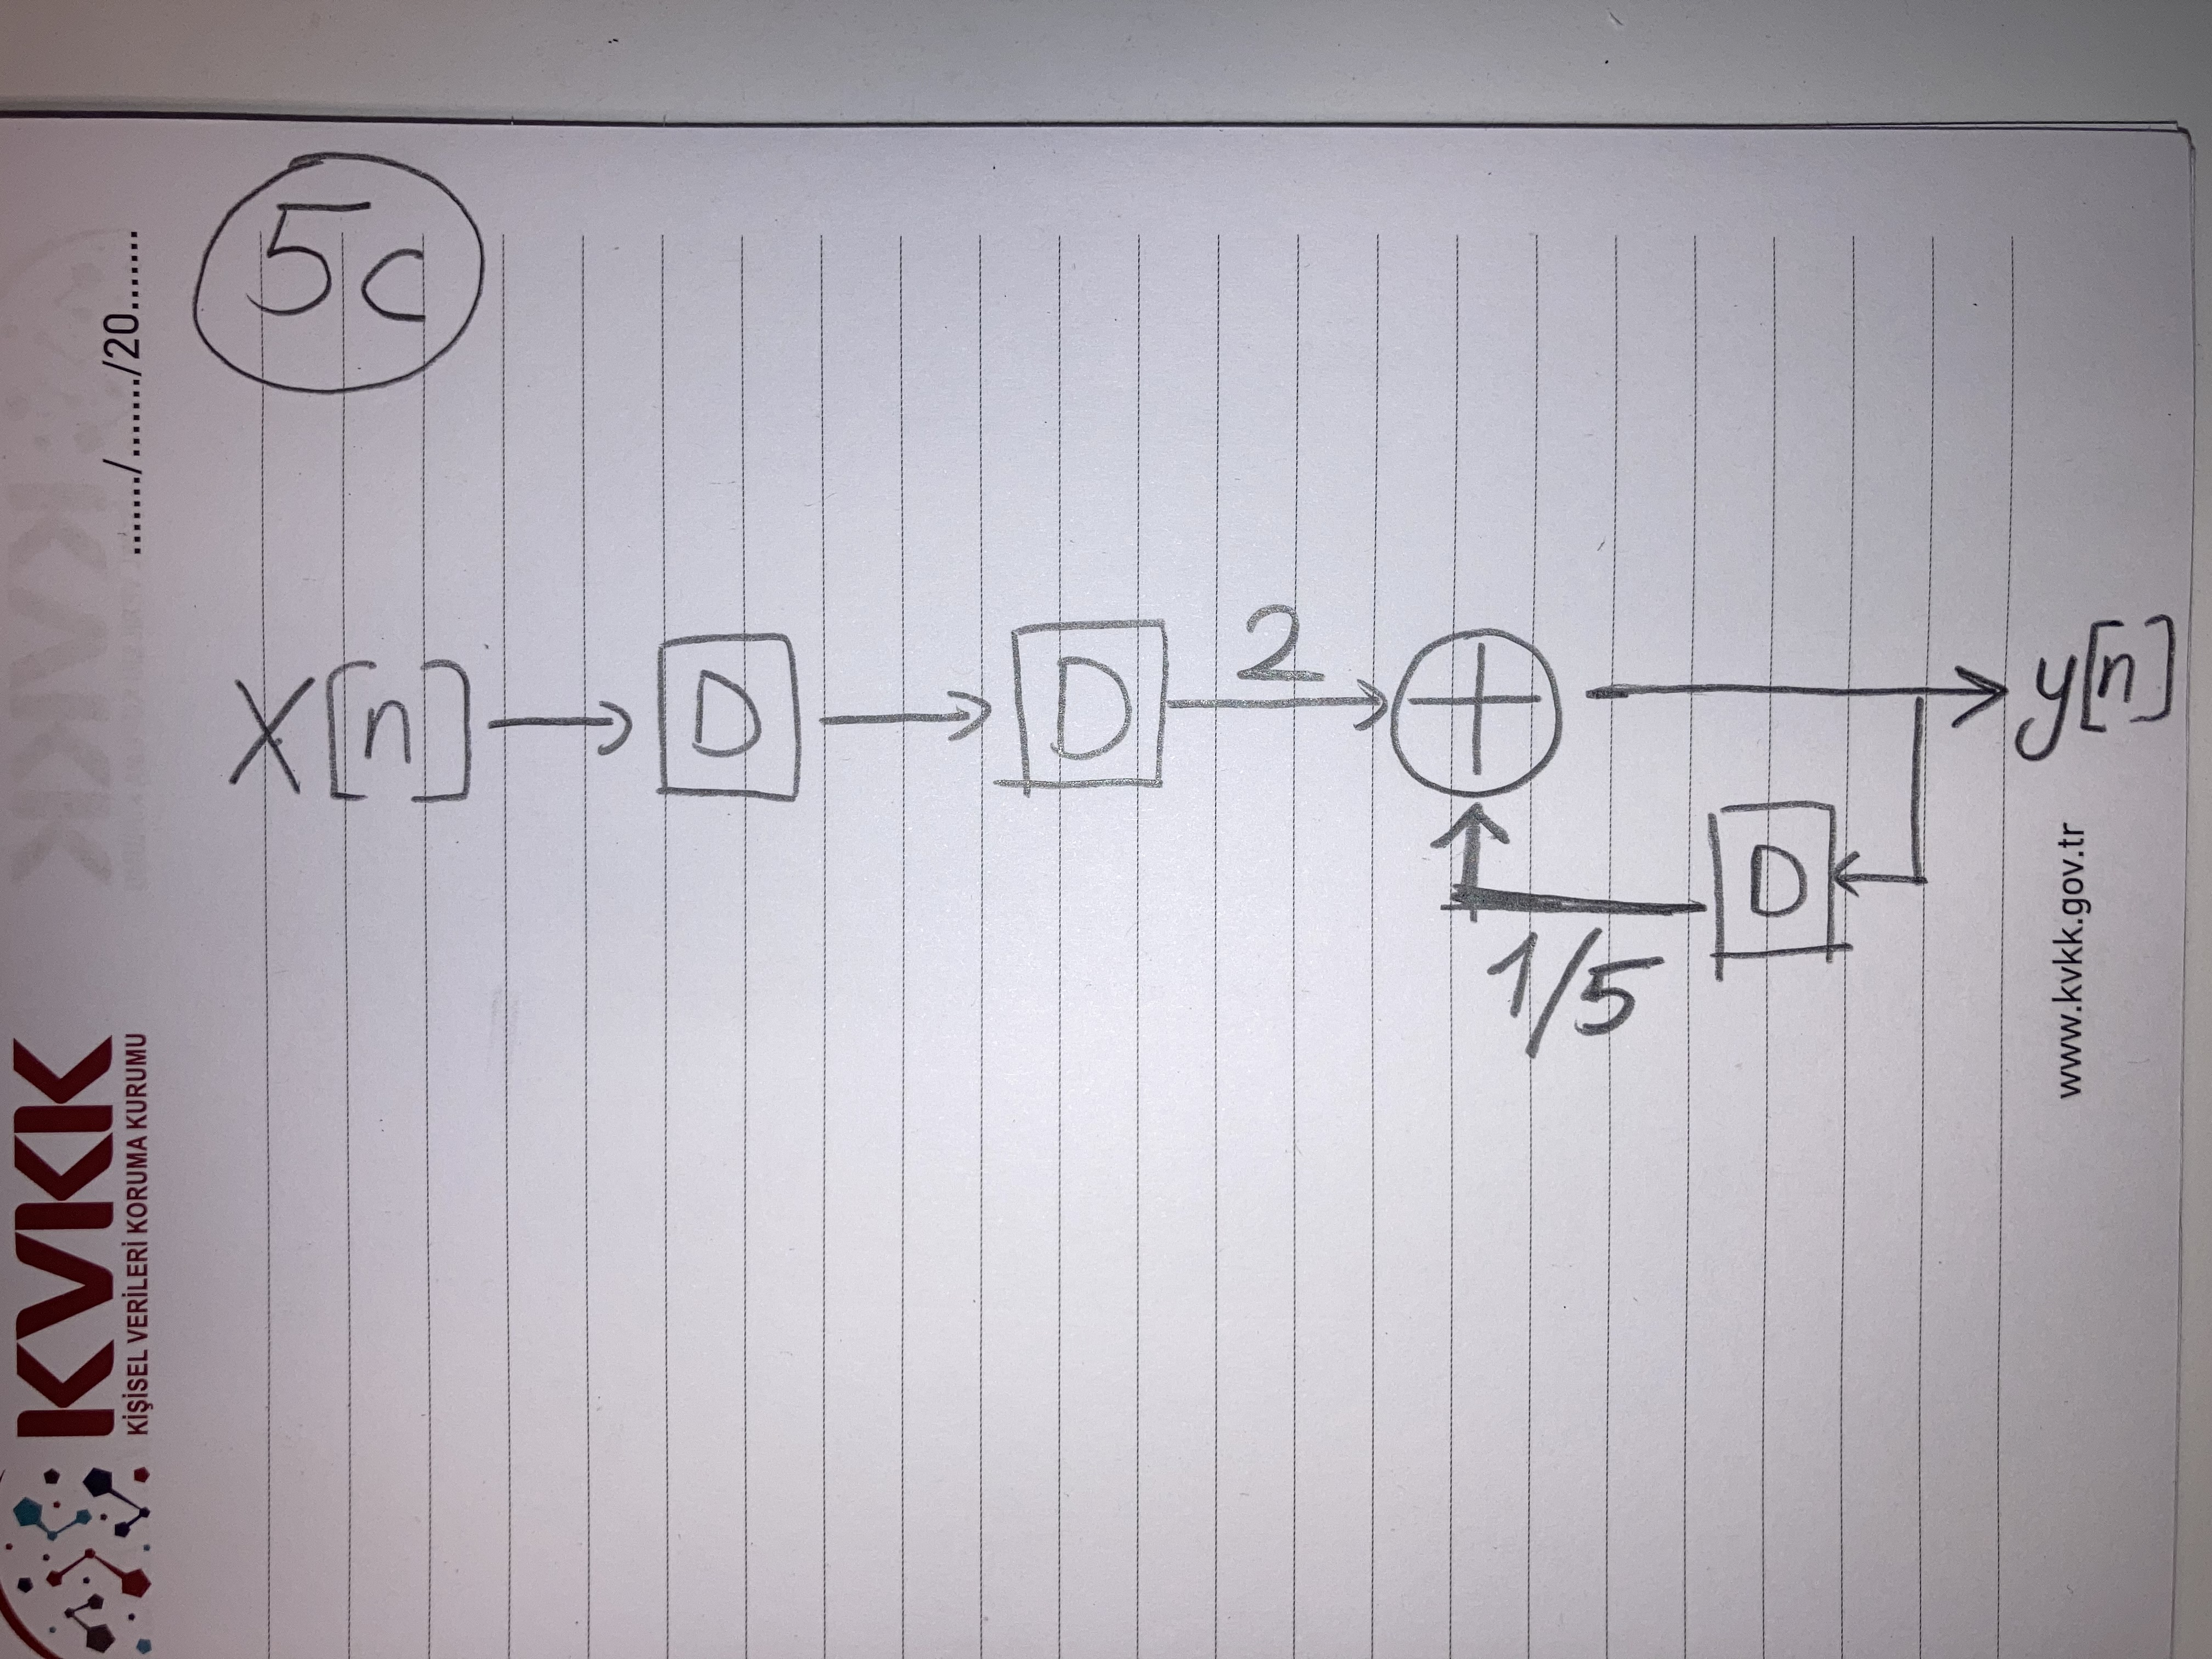
\includegraphics[width=1\linewidth]{q5c.jpg}
        \caption{Solution of Question 5 part c.}
        \label{fig:q5c}
    \end{figure}\vspace{0.3cm}\\
    \end{enumerate} 
    
\item %write the solution of q6
    \begin{enumerate}
    % Write your solutions in the following items.
    \item %write the solution of q6a
    The solution is uploaded as an image in Figure \ref{fig:q6a}, at page \pageref{fig:q6a}.
    \begin{figure}[htbp]
        \centering
        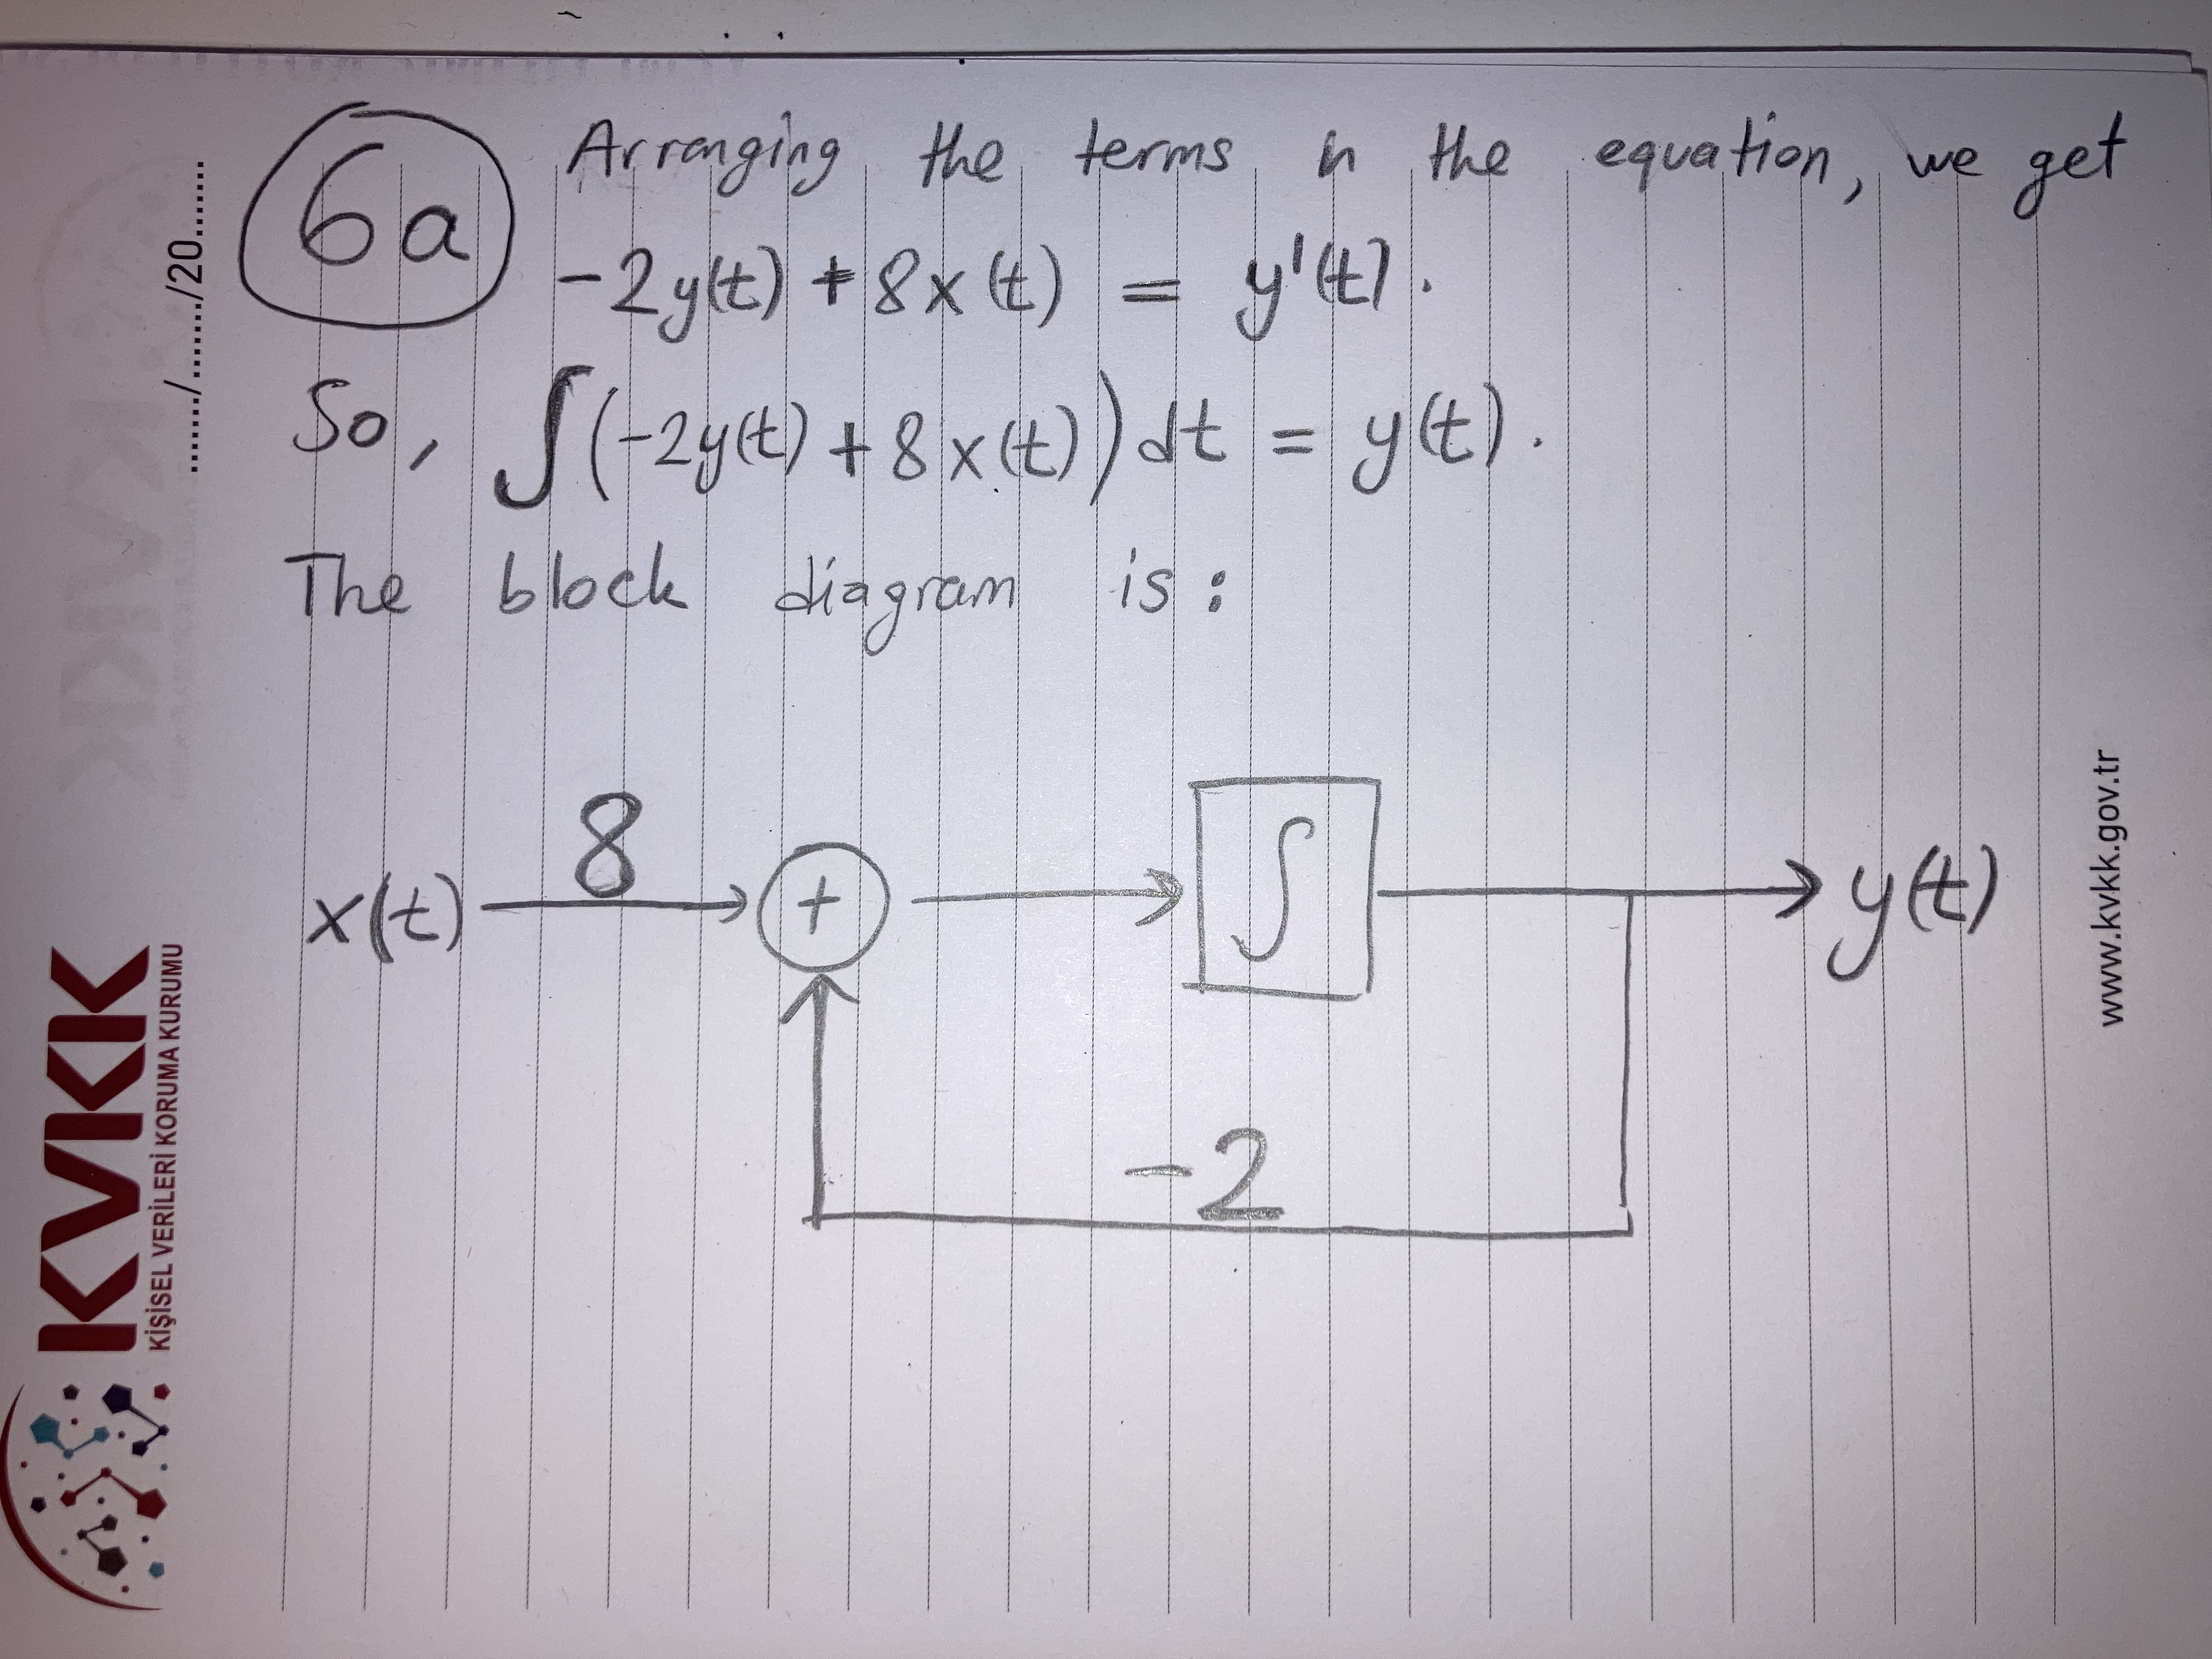
\includegraphics[width=1\linewidth]{q6a.jpg}
        \caption{Solution of Question 6 part a.}
        \label{fig:q6a}
    \end{figure}
    \item %write the solution of q6b
    The solution is uploaded as an image in Figure \ref{fig:q6b}, at page \pageref{fig:q6b}.
    \begin{figure}[htbp]
        \centering
        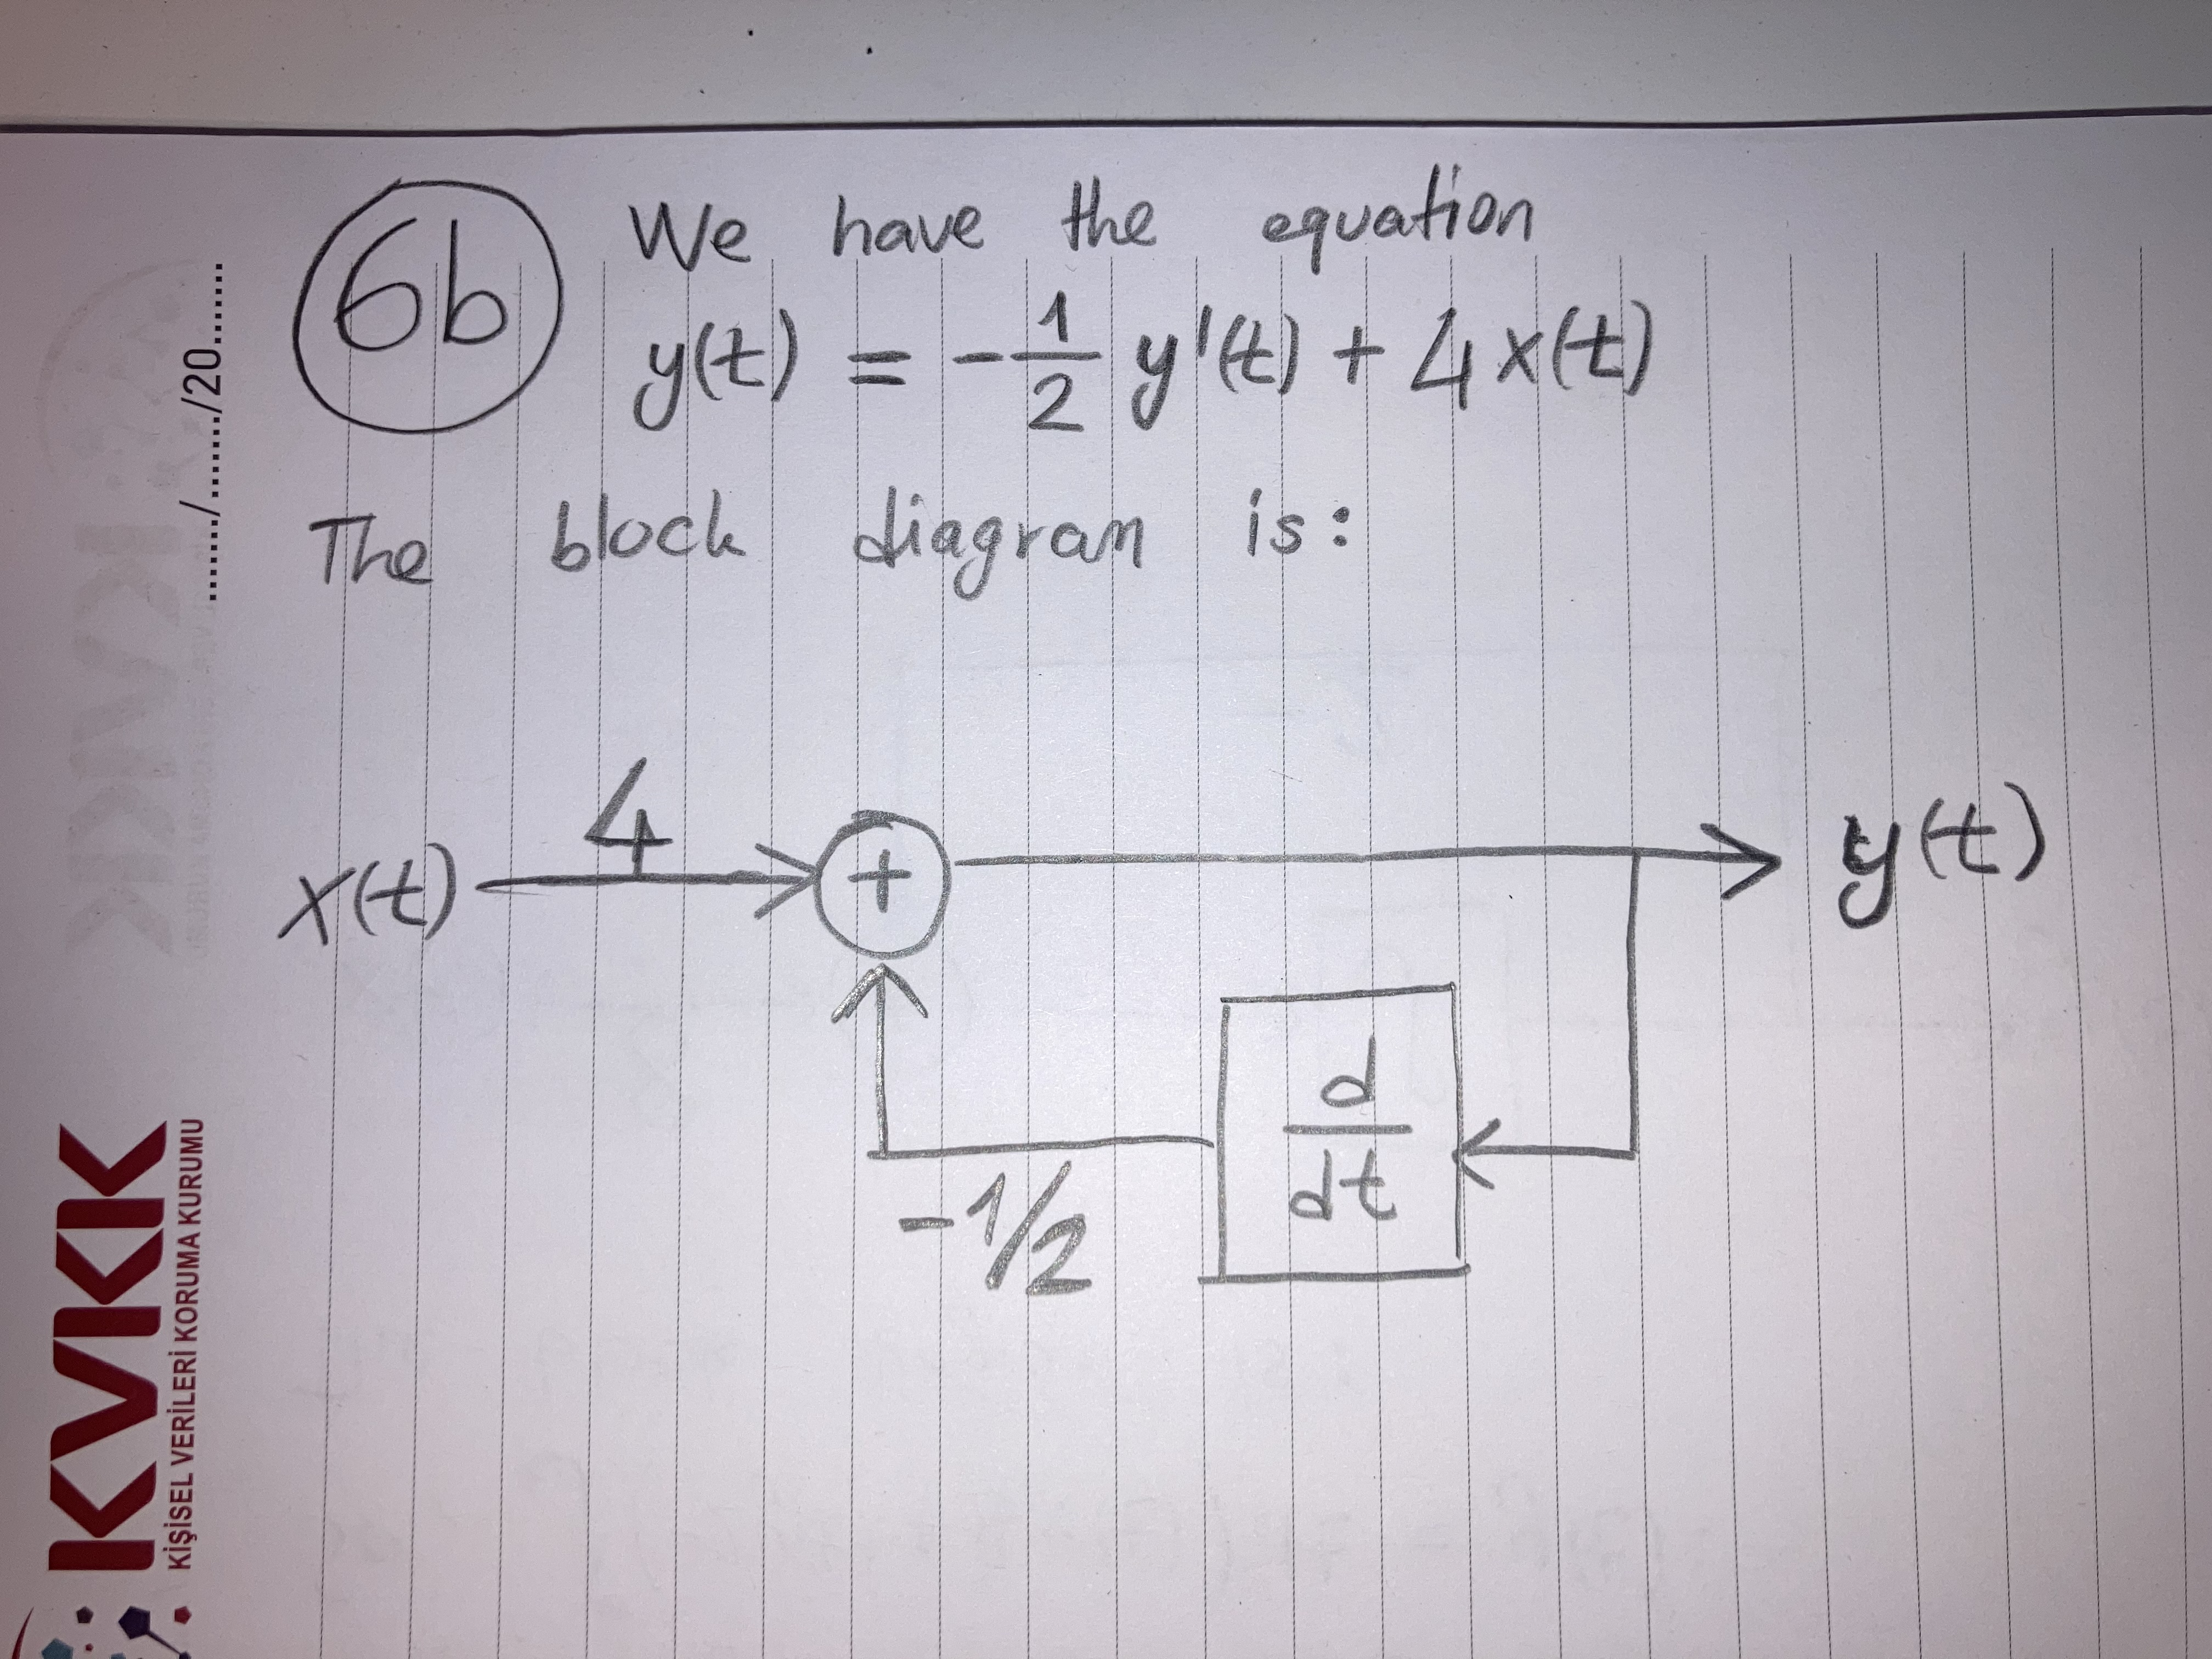
\includegraphics[width=1\linewidth]{q6b.jpg}
        \caption{Solution of Question 6 part b.}
        \label{fig:q6b}
    \end{figure}
    \end{enumerate}
    
\item %write the solution of q7
    Here is the code solution of the introduced task in the question:
    \begin{verbatim}
        import matplotlib.pyplot as plt

        def x(n):
            return 1 if n == 1 else 0
        
        def y(n):
            if n < 0:
                return 0
            return 0.25 * y(n-1) + x(n)
        
        n_samples = 5
        ys = [y(i) for i in range(n_samples)]
        
        plt.scatter(range(n_samples), ys)
        plt.xlabel('n')
        plt.ylabel('y[n]')
        plt.title('Output signal y[n]')
        plt.grid(True)
        plt.show()
    \end{verbatim}
\end{enumerate}


\end{document}
